% Chapter Template

\chapter{Bootloader U-Boot} % Main chapter title

\label{Chapitre 2} % Change X to a consecutive number; for referencing this chapter elsewhere, use \ref{ChapterX}

\lhead{ \emph{Bootloader U-Boot}} % Change X to a consecutive number; this is for the header on each page - perhaps a shortened title

%----------------------------------------------------------------------------------------
%	SECTION 1
%----------------------------------------------------------------------------------------
\section{MMC partitionning}

\subsection{Automated MMC partitionning}

Le tout premier laboratoire était destiné à créer un petit script qui doit permettre d'automatiser la procédure d'installation de la MMC. Voilà directement notre proposition de script :

\begin{lstlisting}[frame=single,style=Console]  % Start your code-block

#!/bin/bash

diskId=$1
specCmd=$2

echo  "--------------- ODROID XU-3 MMC partition utility --------------"
echo  "| 	Written by : Michael Mueller                           |"
echo  "| 	Modified by : Cyrille Savy                             |"
echo  "----------------------------------------------------------------"


# Verification que l'utilisateur est bien root

uid=$(whoami)

if [ "$diskId" == "" ]
then
	echo "./flash_disk.sh <dev_name> [erase] !"
	exit -1
else 	echo  "Writing on device : $diskId" 
fi


if [ "$uid" == "root" ]
then
	if [ "$specCmd" == "erase_all" ]
	then
		echo "Erasing all..."
		dd if=/dev/zero of=$diskId bs=512 seek=1 count=2097152
		sync
	else echo "Writing partition only..."
	fi

	echo "Creating msdos MBR..."
	# First sector: msdos
	parted $diskId mklabel msdos

	echo "Creating bootfs..."
	# create bootfs 64MB
	parted $diskId mkpart primary ext4 131072s 262143s

	echo "Creating rootfs..."
	# create rootfs 256MB
	parted $diskId mkpart primary ext4 262144s 786431s

	echo "Creating usrfs..."
	# create usrfs  256MB
	parted $diskId mkpart primary ext4 786432s 1310719s  
	
	echo "Formatting bootfs..."
	# format with label
 	mkfs.ext4 $diskId"1" -L bootfs

	echo "Formatting rootfs..."
	# format with label
 	mkfs.ext4 $diskId"2" -L rootfs

	echo "Formatting usrfs..."
	# format with label
 	mkfs.ext4 $diskId"3" -L usrfs
	sync

	echo "Copying third-party firmware..."
	#copy firmware & bl1.bin, bl2.bin,tzsw.bin
	dd if=~/workspace/xu3/buildroot/output/images/xu3-bl1.bin of=$diskId bs=512 seek=1  
	dd if=~/workspace/xu3/buildroot/output/images/xu3-bl2.bin of=$diskId bs=512 seek=31 
	dd if=~/workspace/xu3/buildroot/output/images/xu3-tzsw.bin of=$diskId bs=512 seek=719 
	sync

	echo "Copy U-BOOT..."
	#copy u-boot
	dd if=~/workspace/xu3/buildroot/output/images/u-boot.bin of=$diskId bs=512 seek=63 
	sync

	echo "Copy kernel and dtb..."
	mkdir /mnt/bootfs
	mount -t ext4 $diskId"1" /mnt/bootfs
	#copy kernel & flattened device tree
	cp ~/workspace/xu3/buildroot/output/images/uImage /mnt/bootfs/
	cp ~/workspace/xu3/buildroot/output/images/exynos5422-odroidxu3.dtb /mnt/bootfs/ 
	sync
	#unmount filesystem
	umount /mnt/bootfs

	echo "Copy rootfs..."
 	#copy rootfs
	dd if=~/workspace/xu3/buildroot/output/images/rootfs.ext4 of=$diskId"2" bs=512 
	#dd if=~/workspace/xu3/buildroot/output/images/rootfs.ext4 of=$diskId bs=512 seek=262144 
	sync

	echo ""
	echo "DONE WITH SUCCESS! "
	echo ""
	exit 0

else echo "root permission required !";exit -1
fi

\end{lstlisting}

Voici quelques explication pour les grandes lignes de ce scripts : dans premier temps on vérifie que l'on a passé un "device" en paramètre (par exemple "/dev/sdb"). Ensuite vérifie que l'utilisateur possède les droits suffisant ("root"). 
%TODO : Ajouter la suite des explications

\pagebreak
\subsection{MMC File positionning}

Dans cette partie du laboratoire nous avons du essayer de déplacer les divers fichiers sur la carte SD. Nous avons commencé par déplacer "bl1.bin" qui est un premier bootloader. Voilà les commandes utilisées (effacement de la mémoire et réécriture dans une autre zone) :
\begin{lstlisting}[frame=single,style=Console]  % Start your code-block

# BL1
dd if=/dev/zero of=$diskId bs=512 seek=1 count=31
dd if=~/workspace/xu3/buildroot/output/images/xu3-bl1.bin of=$diskId bs=512 seek=17849  # déplacé
\end{lstlisting}

La carte ne fait rien! Évidemment, si le processeur ne trouve pas le "bootloader", il ne peut charger aucun logiciel. 
Nous avons ensuite essayer de déplacer "bl2.bin". Voilà les commandes utilisées (effacement de la mémoire et réécriture dans une autre zone) : 
\begin{lstlisting}[frame=single,style=Console]  % Start your code-block

# BL2
dd if=/dev/zero of=$diskId bs=512 seek=31 count=29
dd if=~/workspace/xu3/buildroot/output/images/xu3-bl2.bin of=$diskId bs=512 seek=17849 # déplacé
\end{lstlisting}

La carte ne fait rien non plus... On peut partir du principe que le premier bootloader à été chargé en mémoire et exécuté et que le deuxième n'étant pas présent n'as pas démarré. Donc le système ne fonctionne pas. 
Nous avons essayé de déplacer la "trustzone". Voilà les commandes utilisées (effacement de la mémoire et réécriture dans une autre zone) : 
\begin{lstlisting}[frame=single,style=Console]  % Start your code-block

#TZ
dd if=/dev/zero of=$diskId bs=512 seek=719 count=512
dd if=~/workspace/xu3/buildroot/output/images/xu3-tzsw.bin of=$diskId bs=512 seek=17849 # déplacé
\end{lstlisting}

Cette fois u-boot démarre. Est-ce normal ou est-ce que la "trust-zone" n'est pas utilisée, nous ne savons pas... Peut-être que nous avons fait des erreurs de manipulations. Essayons encore de déplacer u-boot. 
Voilà les commandes utilisées (effacement de la mémoire et réécriture dans une autre zone) : 

\begin{lstlisting}[frame=single,style=Console]  % Start your code-block

#Uboot
dd if=/dev/zero of=$diskId bs=512 seek=63 count=552
dd if=~/workspace/xu3/buildroot/output/images/u-boot.bin of=$diskId bs=512 seek=17849 # déplacé
\end{lstlisting}

U-boot ne démarre pas (on peut en déduire que c'est logique...)! Par contre le ventilateur s'est mis à tourner, ce qui porte à penser que "bl2.bin" à bien démarré, mais n'as pas trouvé "u-boot".

%TODO Cyrille : à ajouter tes parties -> fait
\begin{lstlisting}[frame=single,style=Console]  % Start your code-block

#Kernel
dd if=/dev/zero of=$diskId bs=512 seek=1263 count=6412
dd if=~/workspace/xu3/buildroot/output/images/uImage of=$diskId bs=512 seek=17849 # déplacé
\end{lstlisting}

\begin{center} 
\hspace{15cm}
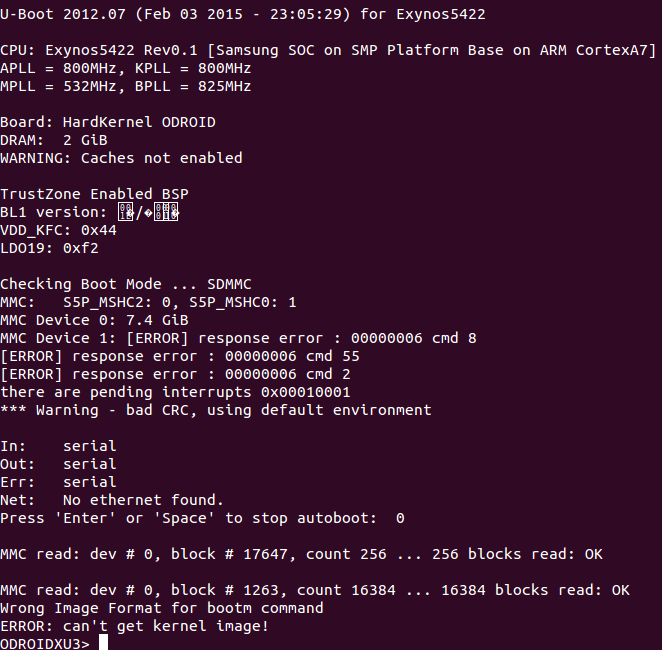
\includegraphics[width=14cm]{deplacer_kernel.png}
\end{center}
\vspace{0.5cm}

Cette fois-ci, logiquement, U-Boot démarre normalement. Mais au moment de charger le noyau linux, il nous dit qu'il n'arrive pas à le trouver (et oui, il n'est plus à l'adresse configurée dans les commandes de boot). Ce qui est rassurant, c'est que U-Boot n'essaie pas de lancer un code sans en vérifier la validité.

\begin{lstlisting}[frame=single,style=Console]  % Start your code-block

#DTB
dd if=/dev/zero of=$diskId bs=512 seek=17647 count=102 # dtb
dd if=~/workspace/xu3/buildroot/output/images/exynos5422-odroidxu3.dtb of=$diskId bs=512 seek=17849 #déplacé 
\end{lstlisting}

\begin{center} 
\hspace{15cm}
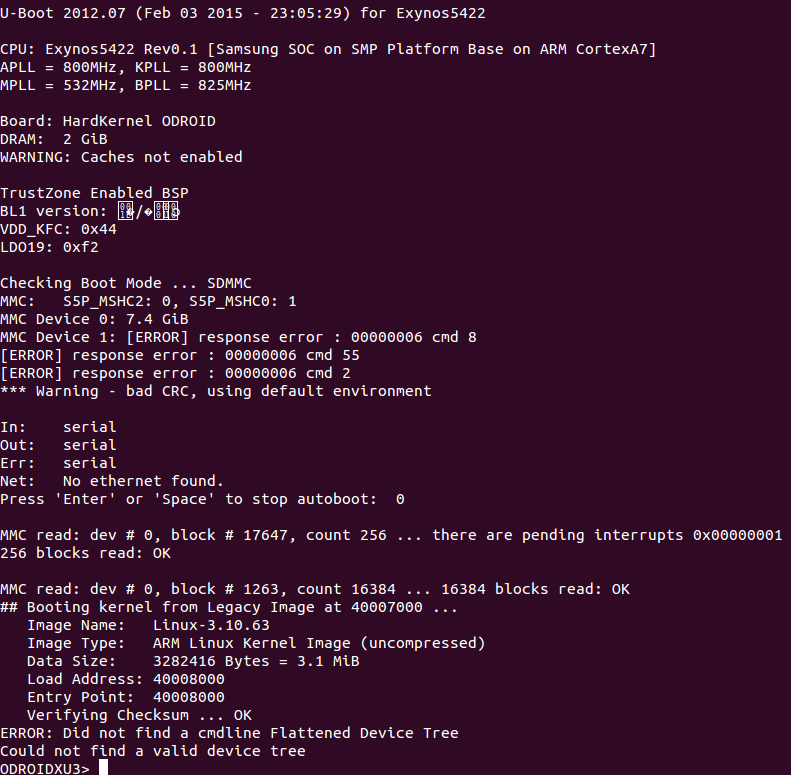
\includegraphics[width=14cm]{deplacer_DTB.png}
\end{center}
\vspace{0.5cm}

Cette fois-ci, U-Boot démarre et arrive à charger charger le noyau linux, trouve que la checksum du noyau est correcte, mais il ne lance pas le noyau car il ne trouve pas un Flattened Device Tree correct.

\pagebreak
\subsection{U-Boot "bootcmds"}
Cette petite section nous a permis de tester différentes commandes possible pour démarrer le noyau Linux.

\subsubsection{bootelf}
Nous avons testé cette commande sans succès (après avoir compilé et généré correctement l'image du noyau Linux). Voici les résulats que nous avons obtenus lors du démarrage :
\begin{center} 
\hspace{15cm}
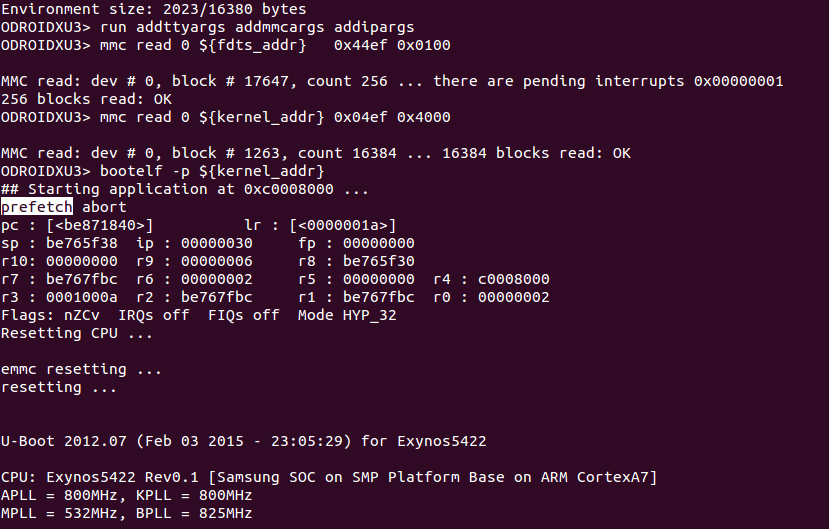
\includegraphics[width=15cm]{bootelf.png}
\end{center}
\vspace{0.5cm}

L'adresse de démarrage du noyau est mal récupérée et le processeur saute à une adresse non valide. Donc il faudrait modifier u-boot pour que cela fonctionne... 

\subsubsection{Bootz}

Cette commande avait l'air de fonctionner, mais une fois le noyau décompressé et que "u-boot" lance le noyau, tout reste figé ! Nous avons trouvé la commande dans le code source sans pourvoir approfondir plus le problème. Il se trouve qu'un offset est mal calculé du à une entête du fichier exécutable.

\subsubsection{Bootp}
Nous n'avons malheureusement pas eu le temps de tester cette commande. Elle utilise le protocole TFTP pour copier et démarrer le noyau Linux.

\pagebreak
\subsubsection{Bootm CRC}

La commande "bootm" permet de tester si le CRC est correct. Voici les tests que nous avons fait. Si le CRC est correcte : 
\begin{center} 
\hspace{15cm}
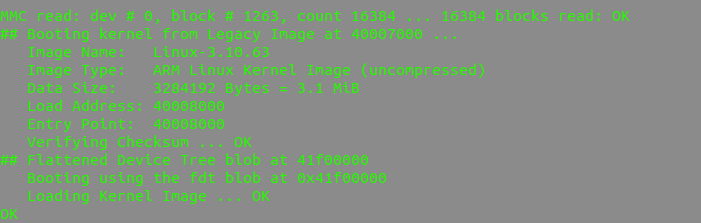
\includegraphics[width=15cm]{CRCOk.png}
\end{center}
\vspace{0.5cm}

En modifiant un bit au hasard, la commande ne devrait pas démarrer :
\begin{center} 
\hspace{15cm}
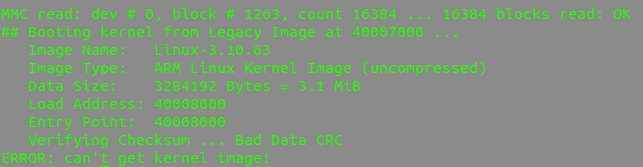
\includegraphics[width=15cm]{badCRC.png}
\end{center}
\vspace{0.5cm}

La commande "bootm" utilise l'algorithme CRC32 pour vérifier l'intégrité. Ce n'est pas la solution idéale à cause des collisions possibles. Il faudrait plutôt une fonction de hashage de type SHA2, voir SHA3 pour les futuriste.

Si on essaye de lancer notre noyau modifié sans contrôle :
\begin{center} 
\hspace{15cm}
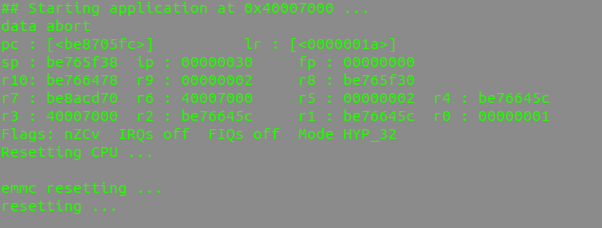
\includegraphics[width=15cm]{CRCPasCheck.png}
\end{center}
\vspace{0.5cm}

Ça plante bien évidemment! Donc, au niveau du "bootloader" c'est important de tester l'intégrité du noyau. L'idéal serait de pouvoir tester à l'aide de signature asymétrique (utilisations de certificats...)

\pagebreak
\section{U-Boot hardening}

Dans cette partie nous allons nous concentrer sur la sécurité d'u-boot. Nous allons voir différentes techniques qui vont nous permettre de consolider le software du bootloader.

\subsection{GCC compilation command line}
Une technique est d'ajouter quelques variables de compilation à notre environnement "buildroot".  

\subsubsection{Debug symbol stripping}
Afin de rendre le "reverse-engineering" un peu plus compliqué, on peut ôter divers symboles de "debug" en supprimant l'option de compilation "-g". Comme demandé, nous l'avons supprimé dans "buildroot" (modification de "config.mk" du dossier "uboot-eiafr"). Voici les options de compilation actuelle : 
\begin{center} 
\hspace{15cm}
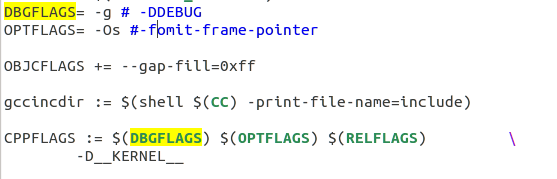
\includegraphics[width=15cm]{Uboot_Hard_Before.png}
\end{center}
\vspace{0.5cm} 

Et après modification (nous avons aussi ajouté la protection de la pile. Voir le sous-chapitre suivant pour les explications) :
\begin{center} 
\hspace{15cm}
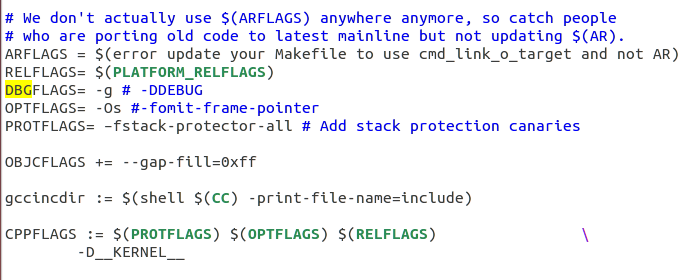
\includegraphics[width=15cm]{Uboot_Hard_After.png}
\end{center}
\vspace{0.5cm} 

Par cette simple manière, nous avons déjà protégé considérablement notre bootloader. Il y a encore une grande quantité de librairies standard qui ne sont pas compilée avec ces deux options. Les symboles de debug permettent de trouver les failles d'un système plus facilement et la non-protection de la pile permet leur exploitations... Donc à ne surtout pas oublier dans les nouvelles applications! 
\pagebreak

\subsubsection{Using canaries}
Comme vu juste précédemment, nous avons ajouté une option de compilation qui permet de protéger la pile : "-fstack--protector-all". \\
Cette option permet de protéger de manière efficace contre les vulnérabilités de type "bufferoverflow" (généralement suite à une vulnérabilité de type "integeroverflow"). \\

Cette vulnérabilité est simple : si la taille d'une écriture dans un tableau  sur la pile n'est pas contrôlée, il y a un risque que l'on réécrive l'adresse de retour de la fonction. C'est par cette méthode que l'on peut injecter un code malin et prendre le contrôle d'un ordinateur. \\
Pour parer à ce problème, on a rajouté entre l'adresse de retour et les variables locale (qui sont sur la pile), une valeur aléatoire qui est contrôlée à la fin de la fonction. On les appelle des "canaris", nom historique reçu des mineurs de charbon qui utilisaient des canaris pour détecter le "grisou" (gaz très explosif...) présent dans les mines. 

Voici un exemple de programme compilé sans et avec cette option. C'est le code "C" identique pour les deux programmes :
\begin{lstlisting}[frame=single,style=C]  % Start your code-block

void func_a(int var)
{
	int loc = var;
	return;
}

int main(void)
{
	func_a(1);
	return 0;
}
\end{lstlisting}

On voit un bête appel de fonction avec une valeur et une variable local. Voici l'assembleur généré pour la fonction "func\_a" :
\begin{lstlisting}[frame=single,style=C]  % Start your code-block

080483fc <main>:
	push   %ebp
	mov    %esp,%ebp
	sub    $0x4,%esp
	
	// Appel de "func_a"
	movl   $0x1,(%esp)
	call   80483ed <func_a>
	... 
080483ed <func_a>:
	// Appel de fonction standard
	push   %ebp
	mov    %esp,%ebp
	sub    $0x10,%esp
	
	// int loc = var
	mov    0x8(%ebp),%eax
	mov    %eax,-0x4(%ebp)
	
	//Retour de la fonction
	nop
	leave  
	ret  
\end{lstlisting}

On voit que la fonction est simple, et qu'aucun contrôle de la pile n'est fait. 

\pagebreak Voyons maintenant avec la protection de la pile ce qu'on obtient :
\begin{lstlisting}[frame=single,style=C]  % Start your code-block

0804846e <main>:
	push   %ebp
	mov    %esp,%ebp
	and    $0xfffffff0,%esp
	sub    $0x20,%esp
	
	// On met le canari sur la pile
	mov    %gs:0x14,%eax // GS = Segment register.
	mov    %eax,0x1c(%esp) 
	
	// EAX = 0
	xor    %eax,%eax
	
	// Appel de la fonction "func_a"
	movl   $0x1,(%esp)
	call   804843d <func_a>
	...
	
0804843d <func_a>:
	push   %ebp
	mov    %esp,%ebp
	sub    $0x28,%esp  // On réserve plus de place
	
	// int loc = var
	mov    0x8(%ebp),%eax
	mov    %eax,-0x1c(%ebp)  // loc est à l'adresse (%EBP) - 0x1C 
	
	// On met le canari sur la pile
	mov    %gs:0x14,%eax  
	mov    %eax,-0xc(%ebp) // Le canari est au dessus des variables. 
	xor    %eax,%eax // Mise à zero d'EAX
	
	mov    -0x1c(%ebp),%eax // EAX = loc 
	mov    %eax,-0x10(%ebp) // On met loc sur la pile juste avant le canari... Pourquoi ??
	nop
	
	// Check si le canari est toujours de la bonne valeur
	mov    -0xc(%ebp),%eax
	xor    %gs:0x14,%eax
	je     804846c <func_a+0x2f>
	call   8048310 <__stack_chk_fail@plt> //Appel de cette fonction si le canari est faux
	leave  
	ret   
\end{lstlisting}

Donc on remarque que le compilateur à rajouté pas mal de lignes pour vérifier que la pile n'as pas été dépassée/écrasée par une action malveillante! 